%%%%%%%%%%%%%%%%%%%%% chapter.tex %%%%%%%%%%%%%%%%%%%%%%%%%%%%%%%%%
%
% sample chapter
%
% Use this file as a template for your own input.
%
%%%%%%%%%%%%%%%%%%%%%%%% Springer-Verlag %%%%%%%%%%%%%%%%%%%%%%%%%%
%\motto{Use the template \emph{chapter.tex} to style the various elements of your chapter content.}
\chapter{Figuras, Tabelas e Diagramas }
\label{intro} % Always give a unique label
% use \chaptermark{}
% to alter or adjust the chapter heading in the running head

% \abstract*{Each chapter should be preceded by an abstract (no more than 200 words) that summarizes the content. The abstract will appear \textit{online} at \url{www.SpringerLink.com} and be available with unrestricted access. This allows unregistered users to read the abstract as a teaser for the complete chapter.
% Please use the 'starred' version of the new \texttt{abstract} command for typesetting the text of the online abstracts (cf. source file of this chapter template \texttt{abstract}) and include them with the source files of your manuscript. Use the plain \texttt{abstract} command if the abstract is also to appear in the printed version of the book.}

Neste cap\'itulo, ser\'a discutido sobre como inserir e formatar figuras, tabelas e diagramas no \LaTeX. Existem diversas prefer\^encias a respeito de formata\c c\~ao e \textit{layout} relacionados a esses elementos, e vamos discutir os mais b\'asicos a fim de trazer uma perspectiva geral para o leitor.

\section{Figuras}
\label{sec:1}
Para a maioria dos tipos de arquivo cient\'ificos, a inserção de figuras \'e essencial. O \LaTeX \ oferece diferentes ferramentas que podem ser utilizadas para inserir figuras e configurá-las para se obter o que precisa. 

\subsection{Inserção de figuras}

Para inserir figuras, devemos utilizar o pacote \verb|\usepackage{graphicx}| no pre\^ambulo do documento.

\noindent O ambiente utilizado para inserir figuras é o ambiente \verb|figure|, delimitado por \verb|\begin{figure}| e \verb|\end{figure}|. Este comando deve ser inserido no corpo do texto e delimita o trecho do c\'odigo onde a figura deve ser inserida juntamente a outros comandos. Além disso, possibilita legendar uma figura produzida no próprio \LaTeX \ ou por outro programa e flutu\'a-la de forma que a perda de espa\c co seja m\'inima.

\noindent O comando \verb|\includegraphics[escala]{nome da figura}| ser\'a utilizado na inser\c c\~ao da figura. Este comando deve ser inserido entre o \verb|\begin{figure}| e \verb|\end{figure}|, onde o par\^ametro \verb|[escala]| entre colchetes indica a porcentagem de escala, por exemplo, escala igual a $1$ implica que a figura terá $100\%$ das suas dimensões originais, escala igual a $0.5$ implica em reduzir a imagem pela metade. Já o parâmetro entre chaves \verb|{nome da figura}| deve conter a localização da figura. Para que a figura seja centralizada, utilizamos o comando \verb|\centering| antes de inclu\'i-la.

\noindent Para adicionar uma legenda \`a figura, deve-se utilizar o comando \verb|\caption{legenda}| logo ap\'os inserir a figura, antes de inserir \verb|\end{figure}|. \\

\begin{trailer}{Exemplo}
\begin{verbatim}
\usepackage{graphicx}

\begin{document}

\noindent Veja na figura a seguir uma superfície determinada 
pela função $f(x,y)=\dfrac{x^2}{5}+\dfrac{y^2}{5}-4$

\begin{figure}[h]
\centering
\includegraphics[scale=0.22]{grafico_tridimensional.png}
\captionsetup{font=small, justification=centering}
\caption{Gr\'afico da fun\c c\~ao $f(x,y)$.}
\end{figure}  

\end{document}
\end{verbatim}
\end{trailer}

\begin{trailer}{Resultado}
 \noindent Veja na figura a seguir uma superfície determinada pela função $f(x,y)=\dfrac{x^2}{5}+\dfrac{y^2}{5}-4$

\begin{figure}[H]
\centering
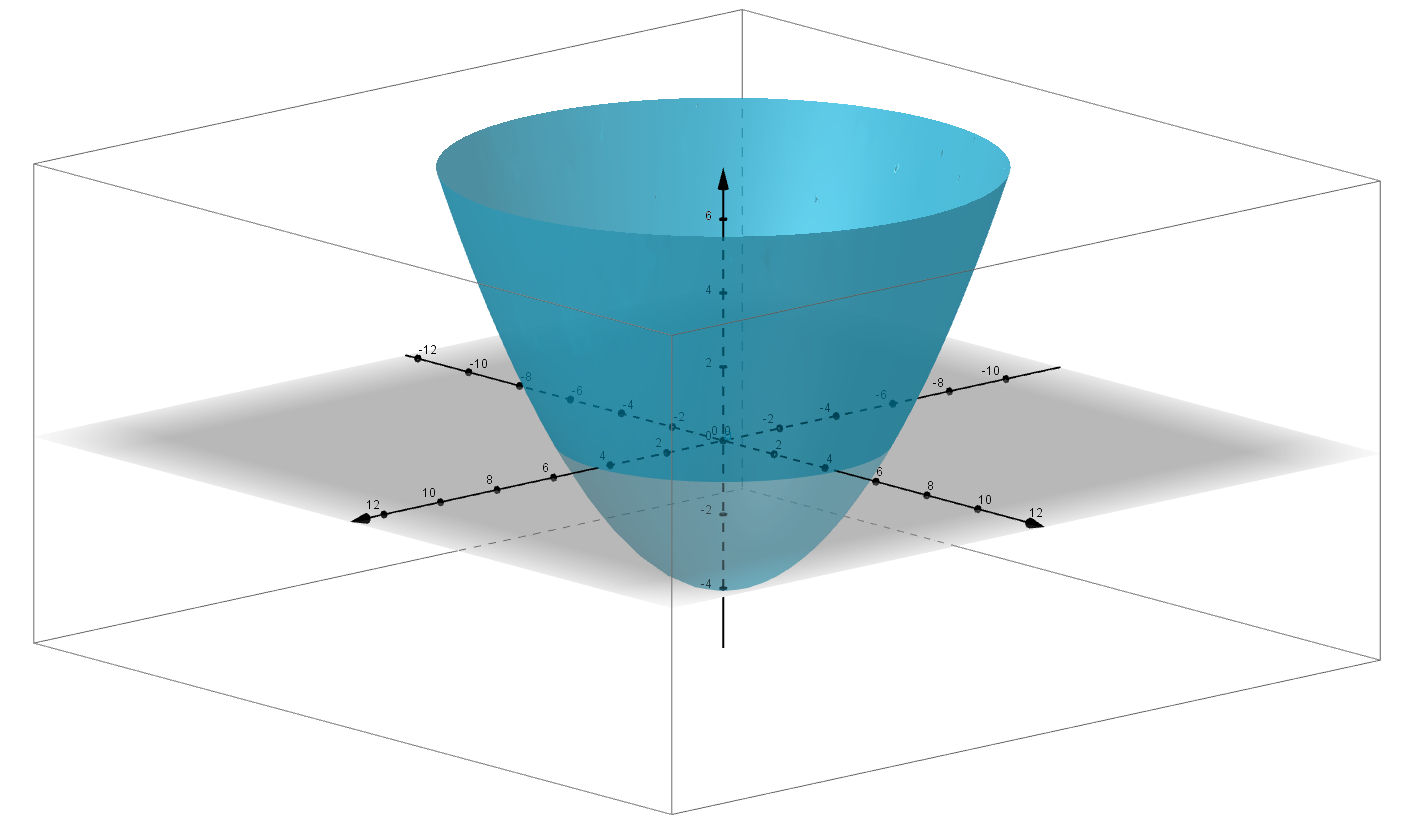
\includegraphics[scale=0.15]{author/grafico_tridim.png}
\captionsetup{font=small, justification=centering}
\caption{Gr\'afico da fun\c c\~ao $f(x,y)$.}
\end{figure}   
\end{trailer}

\subsection{Posicionamento e dimensionamento de figuras}

\noindent O ambiente \verb|figure| tamb\'em permite que possamos reposicionar a figura baseado em alguns comandos. Utilizando \verb|\begin{figure}[onde]|, o argumento “onde” se refere ao local onde deve ser colocada a figura, podendo ser uma combina\c c\~ao das seguintes letras: \\

\begin{itemize}
    \item \textbf{h (here) -} indicará que a figura deve ser inserida exatamente naquele local;
    \item \textbf{t (top) -} indicará que a figura deve ser inserida no topo da próxima página;
    \item \textbf{b (bottom) -}  indicará que a figura deve ser inserida na parte inferior da página;
    \item \textbf{p (page) -} indicará que a figura deve ser inserida em uma p\'agina separada;
    \item \textbf{! -} indicará que devem ser ignorados alguns parâmetros internos e refor\c ca o posicionamento desejado;
    \item \textbf{H -} Caso o \textbf{h} não consiga posicionar uma figura no local desejado nem mesmo com o uso do \textbf{!}, deve-se utilizar o \textbf{H}. Este comando exige o pacote \verb|\usepackage{float}| no preâmbulo. 
\end{itemize}

\noindent Para inclinar uma imagem devemos adicionar o par\^ametro \textit{angle} ao lado do comando \textit{scale} na linha de código \verb|\includegraphics|. O par\^ametro $angle=\theta$ gira a imagem em $\theta$ graus no sentido anti-hor\'ario. Para girar a imagem no sentido hor\'ario, deve-se utilizar um n\'umero negativo. O comando que deve ser utilizado \'e:\\
\vspace{-0.3cm}
\begin{center}
\verb| \includegraphics[scale, angle]{nome da imagem}|.   
\end{center}

\noindent Ao invés de trabalhar apenas alterando a escala das figuras, podemos
redimension\'a-las de outras formas, utilizando como par\^ametros medidas
fixas de largura e/ou altura para a figura. O comando que deve ser utilizado é:
%\vspace{-0.3cm}
\begin{center}
\verb|\includegraphics[width=x cm, height=y cm]{nome da imagem}|,
\end{center}

\noindent onde \textit{widht} indica o comprimento e \textit{height} a altura da figura. Se apenas um dos par\^ametros \textit{width} ou \textit{height} for inserido, o outro ser\'a dimensionado para manter a propor\c c\~ao. 

\subsection{Subfiguras}
Muitas vezes, é necessário incluir várias figuras relacionadas em um mesmo ambiente, como gráficos lado a lado ou imagens que devem ser agrupadas para comparação. A inserção de subfiguras pode ser realizada usando o pacote \texttt{subcaption}, que oferece recursos avançados para criar subfiguras de maneira fácil e personalizável. 

\noindent O pacote \texttt{subcaption} permite criar ambientes de subfiguras dentro de um ambiente \texttt{figure}, permitindo controlar o layout, a legenda e a numeração das subfiguras independentemente. Aqui estão alguns parâmetros comuns usados no ambiente de subfiguras:

\begin{itemize}
    \item \texttt{width}: Define a largura da subfigura. Pode ser especificado em unidades como \verb|cm|.
    \item \texttt{caption}: Define a legenda da subfigura.
    \item \texttt{label}: Define uma etiqueta para referência cruzada.
\end{itemize}

\begin{trailer}{Exemplo}
\begin{verbatim}
\usepackage{graphicx}
\usepackage{subcaption} % Pacote para subfiguras

\begin{document}

\begin{figure}[H]
    \centering

    \begin{subfigure}[b]{0.4\textwidth}
        \centering
        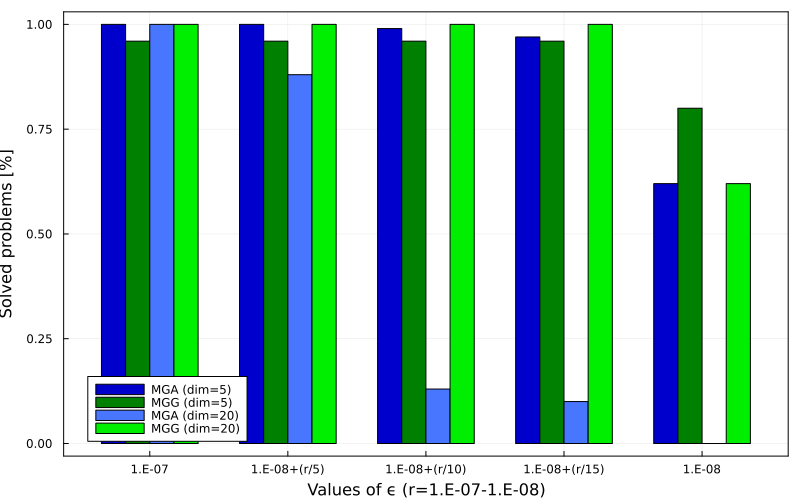
\includegraphics[width=\textwidth]{grafico1.png}
        \caption{Gr\'afico 1.}
    \end{subfigure}
    \hfill
    \begin{subfigure}[b]{0.4\textwidth}
        \centering
        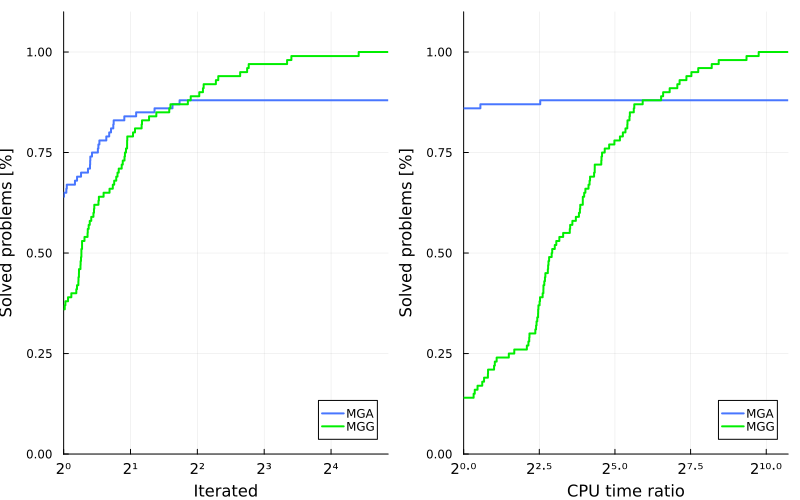
\includegraphics[width=\textwidth]{grafico2.png}
        \caption{Gr\'afico 2.}
    \end{subfigure}
        \begin{subfigure}[b]{0.4\textwidth}
        \centering
        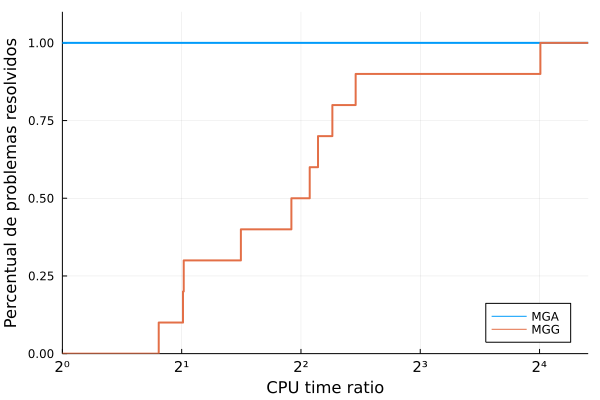
\includegraphics[width=\textwidth]{grafico3.png}
        \caption{Gr\'afico 3.}
    \end{subfigure}

    \caption{An\'alise de gr\'aficos}
    \label{fig:subcaption_example}
\end{figure}

\end{document}
\end{verbatim}   
\end{trailer}

\begin{trailer}{Resultado}
\begin{figure}[H]
    \centering

    \begin{subfigure}[b]{0.4\textwidth}
        \centering
        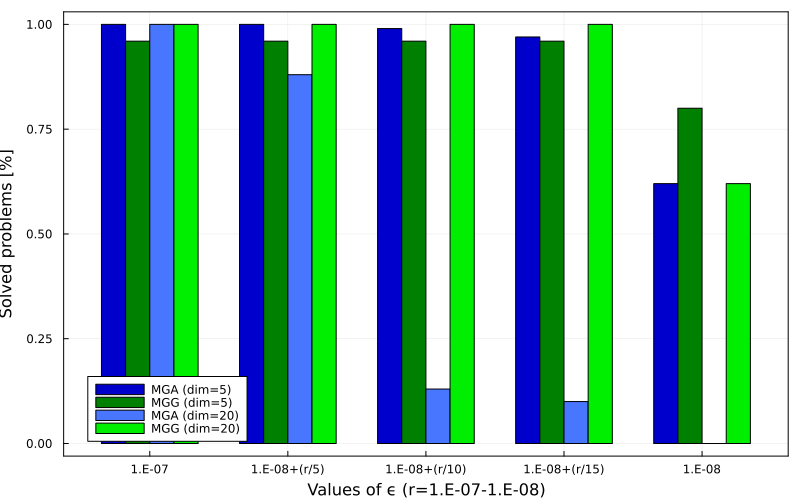
\includegraphics[width=\textwidth]{grafico1.png}
        \caption{Gr\'afico 1.}
    \end{subfigure}
    \hfill
    \begin{subfigure}[b]{0.4\textwidth}
        \centering
        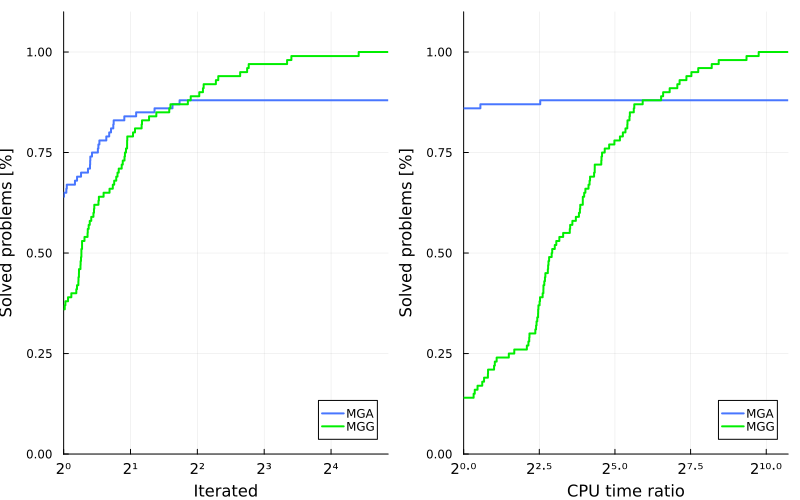
\includegraphics[width=\textwidth]{grafico2.png}
        \caption{Gr\'afico 2.}
    \end{subfigure}
        \begin{subfigure}[b]{0.4\textwidth}
        \centering
        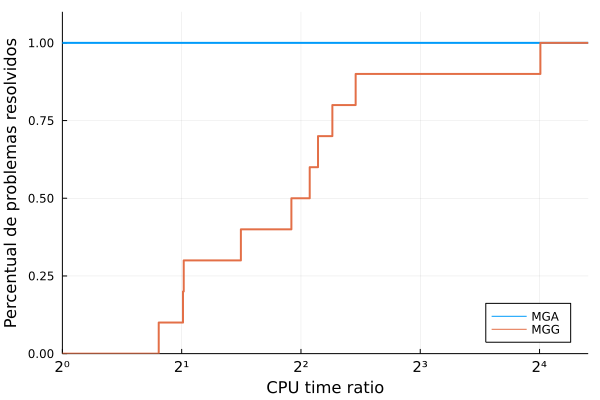
\includegraphics[width=\textwidth]{grafico3.png}
        \caption{Gr\'afico 3.}
    \end{subfigure}

    \caption{An\'alise de gr\'aficos}
    \label{fig:subcaption_example}
\end{figure}    
\end{trailer}

\section{Tabelas}
\label{sec:2}

Tabelas e quadros são elementos essenciais em muitos documentos, pois permitem a organização e apresentação de informações de maneira estruturada. O LaTeX oferece um ambiente poderoso para criar e personalizar tabelas de acordo com suas necessidades.

\subsection{Criação Básica de Tabelas}

Para a cria\c c\~ao de tabelas, deve-se usar o ambiente \texttt{table}. Este ambiente delimita a regi\~ao do c\'odigo onde ser\~ao inseridas as configura\c c\~oes para a tabela. 

\noindent Para inserir a tabela, deve-se usar o ambiente \texttt{tabular} internamente ao ambiente \texttt{table}. Este comando delimita a tabela, para determinar o par\^ametro de n\'umero de colunas. 

\noindent Para o alinhamento do conte\'udo de cada coluna, utilizamos as letras, \textbf{r (right)}, \textbf{l (left)} e \textbf{c (center)} onde \textbf{r} alinha o conteúdo de uma coluna à direita, \textbf{l} à esquerda e
\textbf{c} centraliza. 

\noindent Para determinarmos a quantidade de colunas, basta adicionar um desses par\^ametros para cada coluna e o número de letras de alinhamento ser\'a igual a n\'umero de colunas.

\begin{trailer}{Exemplo}
\begin{verbatim}
\begin{table}[H]
  \centering
  \begin{tabular}{c c}
  célula 1 & célula 2 \\
  célula 3 & célula 4
  \end{tabular}
\end{table}
\end{verbatim}    
\end{trailer}

\begin{trailer}{Resultado}
\vspace{-0.5cm}
\begin{table}
  \centering
  \begin{tabular}{c c}
  célula 1 & célula 2 \\
  célula 3 & célula 4
  \end{tabular}
\end{table}    
\end{trailer}

\subsection{Formatação de Tabelas}
A formatação de tabelas é muito importante para melhorar a legibilidade e a estética. Abaixo estão alguns dos principais comandos de formatação de tabelas.\\

\begin{itemize}
    \item \textbf{Linhas Horizontais:} Use \texttt{\textbackslash hline} para criar linhas horizontais.
    \item \textbf{Colunas Verticais:} Use \texttt{|} entre as letras do argumento do ambiente \texttt{tabular} para criar linhas verticais.
    \item \textbf{Espaçamento:} Use \verb|>{\centering\arraybackslash}p{largura}| para definir espaçamento entre colunas.
\end{itemize}

\begin{trailer}{Exemplo}
\begin{verbatim}
\begin{table}
\centering
\begin{tabular}{|>{\centering\arraybackslash}p{2.5cm}| 
>{\centering\arraybackslash}p{3cm}| 
>{\centering\arraybackslash}p{3.5cm}|}
    \hline
    \textbf{Item} & \textbf{Quantidade} & \textbf{Preço (R\$)} \\
    \hline
    Maçãs & 10 & 2.50 \\
    \hline
    Laranjas & 8 & 3.00 \\
    \hline
    Uvas & 5 & 4.75 \\
    \hline
\end{tabular}
\end{table}
\end{verbatim}   
\end{trailer}

\begin{trailer}{Resultado}
\begin{table}
\centering
\begin{tabular}{|>{\centering\arraybackslash}p{2.5cm}|>{\centering\arraybackslash}p{3cm}|>{\centering\arraybackslash}p{3.5cm}|}
    \hline
    \textbf{Item} & \textbf{Quantidade} & \textbf{Preço (R\$)} \\
    \hline
    Maçãs & 10 & 2.50 \\
    \hline
    Laranjas & 8 & 3.00 \\
    \hline
    Uvas & 5 & 4.75 \\
    \hline
\end{tabular}
\end{table}    
\end{trailer}

\subsection{Mesclagem de Células}

A mesclagem de células pode ser realizada com o pacote \texttt{multirow} para mesclagem vertical e \texttt{multicolumn} para mesclagem horizontal.
\vspace{0.3cm}

\begin{trailer}{Exemplo}
\begin{verbatim}
\begin{table}
\centering
\begin{tabular}{|c|c|c|}
    \hline
    \multicolumn{2}{|c|}{\textbf{Grupo 1}} 
    & \multirow{2}{*}{\textbf{Grupo 2}} \\
    \cline{1-2}
    \textbf{Célula 1} & \textbf{Célula 2} & \\
    \hline
    Dado 1 & Dado 2 & Dado 3 \\
    \hline
    \multirow{2}{*}{\textbf{Células mescladas}} 
    & \multicolumn{2}{c|}{Dado 4} \\
    & \multicolumn{2}{c|}{Dado 5} \\
    \hline
\end{tabular}
\end{table}
\end{verbatim}   
\end{trailer}

\begin{trailer}{Resultado}
 \begin{table}
\centering
\begin{tabular}{|c|c|c|}
    \hline
    \multicolumn{2}{|c|}{\textbf{Grupo 1}} & \multirow{2}{*}{\textbf{Grupo 2}} \\
    \cline{1-2}
    \textbf{Célula 1} & \textbf{Célula 2} & \\
    \hline
    Dado 1 & Dado 2 & Dado 3 \\
    \hline
    \multirow{2}{*}{\textbf{Células mescladas}} & \multicolumn{2}{c|}{Dado 4} \\
    & \multicolumn{2}{c|}{Dado 5} \\
    \hline
\end{tabular}
\end{table}   
\end{trailer}

\subsection{Aparência das tabelas}
V\'arios elementos da tabela podem ser modificados para obter um documento de boa apar\^encia. Pode-se modificar, por exemplo, a espessura, a cor da linha e a cor do plano de fundo das c\'elulas de uma tabela. 

\noindent \'E comum usar duas cores de forma alternada em tabelas para melhorar a legibilidade. Isto pode ser feito em \LaTeX\ com o pacote \texttt{xcolor}, inserindo no pre\^ambulo o comando \verb|{\usepackage[pacote de cores]{xcolor}|. Para inserir as cores, deve-se inserir o comando

\begin{center}
\verb|\rowcolors{\varphi}{cor1! 80! cor2!50 ...}{cor1!70!cor2!40 ...}| 
\end{center}

\noindent antes do ambiente \texttt{tabular}. Esse comando leva tr\^es par\^ametros, cada um dentro de chaves, sendo o primeiro a linha para come\c car a coloriza\c c\~ao, o segundo a cor das linhas \'impares, o terceiro a cor das linhas pares. As cores podem ser misturadas da seguinte forma: o nome da cor seguido de exclama\c c\~ao (exemplo: blue!) e a porcentagem que define sua intensidade em um valor numérico de $0$ a $100$ seguido de exclama\c c\~ao (exemplo: 90!).

% \noindent \textbf{Exemplo:}

% \begin{table}
% \centering
% \rowcolors{1}{}{lightgray}
% \begin{tabular}{|c|c|c|}
%     \hline
%     \textbf{Coluna 1} & \textbf{Coluna 2} & \textbf{Coluna 3} \\
%     \hline
%     Dado 1 & Dado 2 & Dado 3 \\
%     Dado 4 & Dado 5 & Dado 6 \\
%     Dado 7 & Dado 8 & Dado 9 \\
%     \hline
% \end{tabular}
% \caption{Tabela com linhas coloridas alternadas.}
% \end{table}

\noindent Utilizando o comando \verb|\arrayrulecolor|, \'e poss\'ivel colorir as linhas de contorno das tabelas. Este comando deve ser inserido no pre\^ambulo e as cores devem ser inseridas da mesma forma que no pacote \verb|xcolor|.

\noindent Podemos tamb\'em colorir c\'elulas espec\'ificas em uma tabela facilmente atrav\'es do comando \verb|\cellcolor{cores}|. As mesmas observações sobre a sele\c c\~ao de cores mencionadas nos comandos anteriores são v\'alidas para este. Este comando deve ser inserido diretamente na c\'elula que se quer colorir.

\noindent Muitas vezes, a cria\c c\~ao e personaliza\c c\~ao de tabelas no \LaTeX\ podem ser trabalhosas. O site \url{https://www.tablesgenerator.com} \'e uma alternativa para contornar essa dificuldade, pois permite a cria\c c\~ao de tabelas de forma automatizada e gera o c\'odigo em \LaTeX.

\section{Diagramas de Venn}

Os diagramas de Venn s\~ao uma ferramenta visual poderosa para representar rela\c c\~oes entre conjuntos. No \LaTeX, podemos criar esses diagramas usando o pacote \textbf{venndiagram}, que nos permite criar diagramas de Venn de maneira simples e eficaz.

\noindent Primeiramente, o comando \verb|\usepackage{venndiagram}| deve ser inserido no pre\^ambulo.

\noindent Para criar um diagrama de Venn com $2$ conjuntos, pode-se usar o ambiente \verb|venndiagram2sets|. Deve-se usar os comandos \verb|\fillA|, \verb|\fillB| e \verb|\fillAB| para preencher as regi\~oes correspondentes aos conjuntos $A$, $B$ e \`a interse\c c\~ao $AB$, respectivamente.

\begin{trailer}{Exemplo}
\begin{verbatim}
   \begin{venndiagram2sets}    
       \fillA \fillB
   \end{venndiagram2sets}
\end{verbatim}   
\end{trailer}

\begin{trailer}{Resultado}
\begin{center}
   \begin{venndiagram2sets}    
    \fillA \fillB
   \end{venndiagram2sets}
\end{center}   
\end{trailer}

\noindent Para um diagrama com $3$ conjuntos, pode-se utilizar o ambiente \verb|venndiagram3sets| e seguir a mesma estrutura.
%\vspace{0.5cm}

\begin{trailer}{Exemplo}
\begin{verbatim}
   \begin{venndiagram3sets}
       \fillA \fillB \fillC
   \end{venndiagram3sets} 
\end{verbatim}    
\end{trailer}

\begin{trailer}{Resultado}
\begin{center}
   \begin{venndiagram3sets}
    \fillA \fillB \fillC
   \end{venndiagram3sets} 
\end{center}   
\end{trailer}

\noindent O pacote \textbf{venndiagram} oferece várias opções de personalização, incluindo:

\begin{itemize}
    \item \textbf{labelA, labelB, labelC:} Para definir rótulos para os conjuntos.

    \item \textbf{labelOnlyA, labelOnlyB, labelOnlyC:} Para definir rótulos para regiões específicas.

    \item \textbf{labelOnlyAB, labelOnlyAC, labelOnlyBC, labelOnlyABC:} Para rótulos em interseções específicas.
\end{itemize}

\section{Diagramas Comutativos e representa\c c\~ao de Grafos}

\subsection{Diagramas Comutativos}

Um diagrama comutativo \'e uma representa\c c\~ao gr\'afica usada em matem\'atica e outras disciplinas para ilustrar rela\c c\~oes entre objetos e suas transforma\c c\~oes de maneira que o resultado seja independente do caminho escolhido. Em \LaTeX, \'e poss\'ivel criar diagramas comutativos de forma elegante usando pacotes espec\'ificos, como \textbf{tikz-cd}. 

\noindent Para utilizar o pacote \verb|tikz-cd|, você deve inserir no seu pre\^ambulo o comando \verb|\usepackage{tikz-cd}|. O ambiente que ser\'a utilizado \'e o \textbf{tikzcd}. A seguir, mostraremos um exemplo simples.

\begin{trailer}{Exemplo}
\begin{verbatim}
    \begin{tikzcd}
    A \arrow{r}{f} \arrow{d}[swap]{g} & B \\
    C \arrow{ur}[swap]{h}
    \end{tikzcd}
\end{verbatim}   
\end{trailer}

\begin{trailer}{Resultado}
\begin{center}
\begin{tikzcd}
    A \arrow{r}{f} \arrow{d}[swap]{g} & B \\
    C \arrow{ur}[swap]{h}
\end{tikzcd}
\end{center}
\end{trailer}    



\noindent Neste exemplo, temos $3$ objetos: $A$, $B$, $C$ e setas (flechas) que representam as transforma\c c\~oes entre eles. O comando \verb|\arrow| \'e usado para criar flechas e as letras dentro delas representam os nomes das transforma\c c\~oes. A seguir, \'e apresentado um exemplo com $4$ objetos: \\

\begin{trailer}{Exemplo}
\begin{verbatim}
    \begin{tikzcd}
        A \arrow{r}{f} \arrow[swap]{d}{g} & B \arrow{d}{h} \\
        C \arrow{r}{i} & D
    \end{tikzcd}
\end{verbatim}    
\end{trailer}

\begin{trailer}{Resultado}
\begin{center}
\begin{tikzcd}
    A \arrow{r}{f} \arrow[swap]{d}{g} & B \arrow{d}{h} \\
    C \arrow{r}{i} & D
\end{tikzcd}    
\end{center}   
\end{trailer}

\subsection{Grafos}

Os grafos s\~ao uma ferramenta fundamental em matem\'atica e ci\^encia da computa\c c\~ao para representar rela\c c\~oes entre objetos. Em \LaTeX, \'e poss\'ivel criar representações gr\'aficas de grafos usando o pacote \textbf{tikz}, que oferece uma ampla gama de funcionalidades para desenhar grafos personalizados.

\noindent Primeiramente, deve-se inserir no pre\^ambulo o comando \verb|\usepackage{tikz}|.

\noindent Aqui est\~ao alguns conceitos e comandos b\'asicos para a constru\c c\~ao de grafos usando o \textbf{tikz}:

\begin{itemize}
    \item \textbf{Definindo um ambiente de grafo:} Para criar um ambiente para o seu grafo, use o ambiente \textbf{tikzpicture};

    \item \textbf{N\'os (V\'ertices):} Para adicionar n\'os ao seu grafo, use o comando \verb|\node| seguido das coordenadas do n\'o e do nome do n\'o;

    \item \textbf{Arestas:} Para criar arestas entre os n\'os, use o comando \verb|\draw| seguido das coordenadas dos n\'os de origem e destino;
\end{itemize}

\begin{trailer}{Exemplo}
\begin{verbatim}
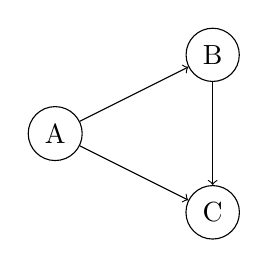
\begin{tikzpicture}
  \node[draw, circle] (A) at (0,0) {A};
  \node[draw, circle] (B) at (2,1) {B};
  \node[draw, circle] (C) at (2,-1) {C};
  
  \draw[->] (A) -- (B);
  \draw[->] (A) -- (C);
  \draw[->] (B) -- (C);
\end{tikzpicture} 
\end{verbatim}    
\end{trailer}

\begin{trailer}{Resultado}
\begin{center}
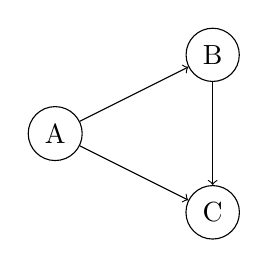
\begin{tikzpicture}
  \node[draw, circle] (A) at (0,0) {A};
  \node[draw, circle] (B) at (2,1) {B};
  \node[draw, circle] (C) at (2,-1) {C};
  
  \draw[->] (A) -- (B);
  \draw[->] (A) -- (C);
  \draw[->] (B) -- (C);
\end{tikzpicture}    
\end{center}   
\end{trailer}

\noindent Abaixo segue um exemplo de um grafo com $4$ n\'os:

\begin{trailer}{Exemplo}
\begin{verbatim}
 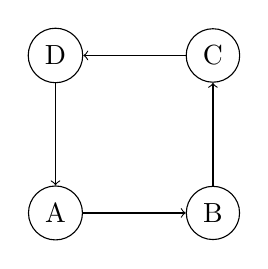
\begin{tikzpicture}
    \node[draw, circle] (A) at (0, 0) {A};
    \node[draw, circle] (B) at (2, 0) {B};
    \node[draw, circle] (C) at (2, 2) {C};
    \node[draw, circle] (D) at (0, 2) {D};

    \draw[->] (A) -- (B);
    \draw[->] (B) -- (C);
    \draw[->] (C) -- (D);
    \draw[->] (D) -- (A);
\end{tikzpicture}   
\end{verbatim}    
\end{trailer}

\begin{trailer}{Resultado}
\begin{center}
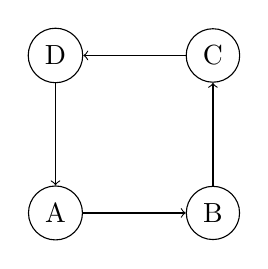
\begin{tikzpicture}
    \node[draw, circle] (A) at (0, 0) {A};
    \node[draw, circle] (B) at (2, 0) {B};
    \node[draw, circle] (C) at (2, 2) {C};
    \node[draw, circle] (D) at (0, 2) {D};

    \draw[->] (A) -- (B);
    \draw[->] (B) -- (C);
    \draw[->] (C) -- (D);
    \draw[->] (D) -- (A);
\end{tikzpicture}     
\end{center}
\end{trailer}

\noindent O \textbf{tikz} permite que você crie grafos mais complexos com diferentes estilos de arestas, cores, formas e tamanhos de n\'os. Voc\^e pode personalizar ainda mais o seu grafo para atender \`as suas necessidades espec\'ificas.

\subsection{Exerc\'icios}

\begin{prob}
    
\end{prob}
\begin{table}[h]
\centering
\caption{Minha Tabela Exemplar}
\label{tab:exemplo}
\begin{tabular}{|c|c|c|c|c|}
\hline
Cabeçalho 1 & Cabeçalho 2 & Cabeçalho 3 & Cabeçalho 4 & Cabeçalho 5 \\ \hline
Dado 1,1 & Dado 1,2 & Dado 1,3 & Dado 1,4 & Dado 1,5 \\ \hline
Dado 2,1 & Dado 2,2 & Dado 2,3 & Dado 2,4 & Dado 2,5 \\ \hline
Dado 3,1 & Dado 3,2 & Dado 3,3 & Dado 3,4 & Dado 3,5 \\ \hline
Dado 4,1 & Dado 4,2 & Dado 4,3 & Dado 4,4 & Dado 4,5 \\ \hline
Dado 5,1 & Dado 5,2 & Dado 5,3 & Dado 5,4 & Dado 5,5 \\ \hline
\end{tabular}
\end{table}

\begin{prob}
    
\end{prob}
\begin{table}[h]
\centering
\caption{Tabela com Mesclagem de Células}
\label{tab:mesclagem}
\begin{tabular}{|c|c|c|c|c|}
\hline
\multicolumn{2}{|c|}{Mesclado 2x1} & Cabeçalho 3 & \multicolumn{2}{c|}{Mesclado 1x2} \\ \hline
Cabeçalho 1 & Cabeçalho 2 & \multirow{2}{*}{Mesclado 2x1} & Cabeçalho 4 & Cabeçalho 5 \\ \cline{1-2} \cline{4-5}
Dado 1,1 & Dado 1,2 & & Dado 1,4 & Dado 1,5 \\ \hline
Dado 2,1 & Dado 2,2 & Dado 2,3 & Dado 2,4 & Dado 2,5 \\ \hline
Dado 3,1 & Dado 3,2 & Dado 3,3 & Dado 3,4 & Dado 3,5 \\ \hline
\end{tabular}
\end{table}

% \section{Conclusão}

%As figuras, tabelas e quadros são elementos cruciais para apresentar informações de maneira organizada e eficaz. O LaTeX oferece uma ampla gama de opções e pacotes para personalizar cada um desses elementos de maneira que atendam às necessidades do seu documento.


%%%%%%%%%%%%%%%%%%%%%%%%% referenc.tex %%%%%%%%%%%%%%%%%%%%%%%%%%%%%%
% sample references
% %
% Use this file as a template for your own input.
%
%%%%%%%%%%%%%%%%%%%%%%%% Springer-Verlag %%%%%%%%%%%%%%%%%%%%%%%%%%
%
% BibTeX users please use
% \bibliographystyle{}
% \bibliography{}
%
\biblstarthook{In view of the parallel print and (chapter-wise) online publication of your book at \url{www.springerlink.com} it has been decided that -- as a genreral rule --  references should be sorted chapter-wise and placed at the end of the individual chapters. However, upon agreement with your contact at Springer you may list your references in a single seperate chapter at the end of your book. Deactivate the class option \texttt{sectrefs} and the \texttt{thebibliography} environment will be put out as a chapter of its own.\\\indent
References may be \textit{cited} in the text either by number (preferred) or by author/year.\footnote{Make sure that all references from the list are cited in the text. Those not cited should be moved to a separate \textit{Further Reading} section or chapter.} If the citatiion in the text is numbered, the reference list should be arranged in ascending order. If the citation in the text is author/year, the reference list should be \textit{sorted} alphabetically and if there are several works by the same author, the following order should be used:
\begin{enumerate}
\item all works by the author alone, ordered chronologically by year of publication
\item all works by the author with a coauthor, ordered alphabetically by coauthor
\item all works by the author with several coauthors, ordered chronologically by year of publication.
\end{enumerate}
The \textit{styling} of references\footnote{Always use the standard abbreviation of a journal's name according to the ISSN \textit{List of Title Word Abbreviations}, see \url{http://www.issn.org/en/node/344}} depends on the subject of your book:
\begin{itemize}
\item The \textit{two} recommended styles for references in books on \textit{mathematical, physical, statistical and computer sciences} are depicted in ~\cite{science-contrib, science-online, science-mono, science-journal, science-DOI} and ~\cite{phys-online, phys-mono, phys-journal, phys-DOI, phys-contrib}.
\item Examples of the most commonly used reference style in books on \textit{Psychology, Social Sciences} are~\cite{psysoc-mono, psysoc-online,psysoc-journal, psysoc-contrib, psysoc-DOI}.
\item Examples for references in books on \textit{Humanities, Linguistics, Philosophy} are~\cite{humlinphil-journal, humlinphil-contrib, humlinphil-mono, humlinphil-online, humlinphil-DOI}.
\item Examples of the basic Springer style used in publications on a wide range of subjects such as \textit{Computer Science, Economics, Engineering, Geosciences, Life Sciences, Medicine, Biomedicine} are ~\cite{basic-contrib, basic-online, basic-journal, basic-DOI, basic-mono}. 
\end{itemize}
}

\begin{thebibliography}{99.}%
% and use \bibitem to create references.
%
% Use the following syntax and markup for your references if 
% the subject of your book is from the field 
% "Mathematics, Physics, Statistics, Computer Science"
%
% Contribution 
\bibitem{science-contrib} Broy, M.: Software engineering --- from auxiliary to key technologies. In: Broy, M., Dener, E. (eds.) Software Pioneers, pp. 10-13. Springer, Heidelberg (2002)
%
% Online Document
\bibitem{science-online} Dod, J.: Effective substances. In: The Dictionary of Substances and Their Effects. Royal Society of Chemistry (1999) Available via DIALOG. \\
\url{http://www.rsc.org/dose/title of subordinate document. Cited 15 Jan 1999}
%
% Monograph
\bibitem{science-mono} Geddes, K.O., Czapor, S.R., Labahn, G.: Algorithms for Computer Algebra. Kluwer, Boston (1992) 
%
% Journal article
\bibitem{science-journal} Hamburger, C.: Quasimonotonicity, regularity and duality for nonlinear systems of partial differential equations. Ann. Mat. Pura. Appl. \textbf{169}, 321--354 (1995)
%
% Journal article by DOI
\bibitem{science-DOI} Slifka, M.K., Whitton, J.L.: Clinical implications of dysregulated cytokine production. J. Mol. Med. (2000) doi: 10.1007/s001090000086 
%
\bigskip

% Use the following (APS) syntax and markup for your references if 
% the subject of your book is from the field 
% "Mathematics, Physics, Statistics, Computer Science"
%
% Online Document
\bibitem{phys-online} J. Dod, in \textit{The Dictionary of Substances and Their Effects}, Royal Society of Chemistry. (Available via DIALOG, 1999), 
\url{http://www.rsc.org/dose/title of subordinate document. Cited 15 Jan 1999}
%
% Monograph
\bibitem{phys-mono} H. Ibach, H. L\"uth, \textit{Solid-State Physics}, 2nd edn. (Springer, New York, 1996), pp. 45-56 
%
% Journal article
\bibitem{phys-journal} S. Preuss, A. Demchuk Jr., M. Stuke, Appl. Phys. A \textbf{61}
%
% Journal article by DOI
\bibitem{phys-DOI} M.K. Slifka, J.L. Whitton, J. Mol. Med., doi: 10.1007/s001090000086
%
% Contribution 
\bibitem{phys-contrib} S.E. Smith, in \textit{Neuromuscular Junction}, ed. by E. Zaimis. Handbook of Experimental Pharmacology, vol 42 (Springer, Heidelberg, 1976), p. 593
%
\bigskip
%
% Use the following syntax and markup for your references if 
% the subject of your book is from the field 
% "Psychology, Social Sciences"
%
%
% Monograph
\bibitem{psysoc-mono} Calfee, R.~C., \& Valencia, R.~R. (1991). \textit{APA guide to preparing manuscripts for journal publication.} Washington, DC: American Psychological Association.
%
% Online Document
\bibitem{psysoc-online} Dod, J. (1999). Effective substances. In: The dictionary of substances and their effects. Royal Society of Chemistry. Available via DIALOG. \\
\url{http://www.rsc.org/dose/Effective substances.} Cited 15 Jan 1999.
%
% Journal article
\bibitem{psysoc-journal} Harris, M., Karper, E., Stacks, G., Hoffman, D., DeNiro, R., Cruz, P., et al. (2001). Writing labs and the Hollywood connection. \textit{J Film} Writing, 44(3), 213--245.
%
% Contribution 
\bibitem{psysoc-contrib} O'Neil, J.~M., \& Egan, J. (1992). Men's and women's gender role journeys: Metaphor for healing, transition, and transformation. In B.~R. Wainrig (Ed.), \textit{Gender issues across the life cycle} (pp. 107--123). New York: Springer.
%
% Journal article by DOI
\bibitem{psysoc-DOI}Kreger, M., Brindis, C.D., Manuel, D.M., Sassoubre, L. (2007). Lessons learned in systems change initiatives: benchmarks and indicators. \textit{American Journal of Community Psychology}, doi: 10.1007/s10464-007-9108-14.
%
%
% Use the following syntax and markup for your references if 
% the subject of your book is from the field 
% "Humanities, Linguistics, Philosophy"
%
\bigskip
%
% Journal article
\bibitem{humlinphil-journal} Alber John, Daniel C. O'Connell, and Sabine Kowal. 2002. Personal perspective in TV interviews. \textit{Pragmatics} 12:257--271
%
% Contribution 
\bibitem{humlinphil-contrib} Cameron, Deborah. 1997. Theoretical debates in feminist linguistics: Questions of sex and gender. In \textit{Gender and discourse}, ed. Ruth Wodak, 99--119. London: Sage Publications.
%
% Monograph
\bibitem{humlinphil-mono} Cameron, Deborah. 1985. \textit{Feminism and linguistic theory.} New York: St. Martin's Press.
%
% Online Document
\bibitem{humlinphil-online} Dod, Jake. 1999. Effective substances. In: The dictionary of substances and their effects. Royal Society of Chemistry. Available via DIALOG. \\
http://www.rsc.org/dose/title of subordinate document. Cited 15 Jan 1999
%
% Journal article by DOI
\bibitem{humlinphil-DOI} Suleiman, Camelia, Daniel C. O'Connell, and Sabine Kowal. 2002. `If you and I, if we, in this later day, lose that sacred fire...': Perspective in political interviews. \textit{Journal of Psycholinguistic Research}. doi: 10.1023/A:1015592129296.
%
%
%
\bigskip
%
%
% Use the following syntax and markup for your references if 
% the subject of your book is from the field 
% "Computer Science, Economics, Engineering, Geosciences, Life Sciences"
%
%
% Contribution 
\bibitem{basic-contrib} Brown B, Aaron M (2001) The politics of nature. In: Smith J (ed) The rise of modern genomics, 3rd edn. Wiley, New York 
%
% Online Document
\bibitem{basic-online} Dod J (1999) Effective Substances. In: The dictionary of substances and their effects. Royal Society of Chemistry. Available via DIALOG. \\
\url{http://www.rsc.org/dose/title of subordinate document. Cited 15 Jan 1999}
%
% Journal article by DOI
\bibitem{basic-DOI} Slifka MK, Whitton JL (2000) Clinical implications of dysregulated cytokine production. J Mol Med, doi: 10.1007/s001090000086
%
% Journal article
\bibitem{basic-journal} Smith J, Jones M Jr, Houghton L et al (1999) Future of health insurance. N Engl J Med 965:325--329
%
% Monograph
\bibitem{basic-mono} South J, Blass B (2001) The future of modern genomics. Blackwell, London 
%
\end{thebibliography}

